\documentclass[11pt]{article}
\usepackage[utf8]{inputenc}
\usepackage[czech]{babel}
\usepackage{a4wide}
\usepackage{graphicx}

\newcommand{\labtitle}[4]{
	\begin{titlepage}
		\begin{center}
			\mbox{} \\[4cm]
			{\huge {#1}} \\[2cm]
			{\Large #2}  % \\[.2cm]
			{\large #3 } \\[.7cm]
			{\normalsize měřeno #4}
		\end{center}
	\end{titlepage}
}


\begin{document}

% -- title page -- %
\labtitle{Studium Geigerova-M\"ullerova počítače pro záření gama}
 {Tomáš Maršálek}
 {(A10B0632P)}
 {14.\,listopadu 2011}
% -- title page -- %

\section{Měřící potřeby a přístroje}
přístroj pro měření radioaktivního záření ROBOTRON 20 046, Geiger-M\"ullerův
počítač pro záření gama, dva zářiče $^{60}$Co o přibližně stejné aktivitě

\section{Naměřené hodnoty}
\subsection{Charakteristika}
Všechna měření probíhala 100 vteřin. Než počítač začal registrovat impulsy,
velikost intervalu mezi měřeními byla 20V, poté 40V. \\

\begin{center}
\begin{tabular}{|c|c|c|c|}
\hline
U [V] & počet impulzů [imp] & četnost [imp/min] & odchylka [imp/min]\\
\hline
340 & 0   & 0      & 0 \\
360 & 158 & 94.8   & 7.5  \\
400 & 167 & 100.2  & 7.8  \\
440 & 152 & 91.2   & 7.4  \\
480 & 162 & 97.2   & 7.6  \\
520 & 165 & 99.0   & 7.7  \\
560 & 149 & 89.4   & 7.3  \\
600 & 165 & 99.0   & 7.7  \\
640 & 178 & 106.8  & 8.0  \\
680 & 161 & 96.6   & 7.6  \\
720 & 198 & 118.8  & 8.5  \\
760 & 229 & 137.4  & 9.1  \\
\hline
\end{tabular}
\end{center}

\vspace{.5cm}
\subsection{Rozlišovací doba}
Vzorky: \\

\begin{center}
\begin{tabular}{|r|c|c|}
\hline
číslo & 1 & 2 \\
\hline
typ   & radionuklid $^{60}$Co & radionuklid $^{60}$Co \\
číslo etalonu & 099-01 & 099-03 \\
počáteční aktivita [kBq] & 185.10 & 185.90 \\
aktivita ke dni měření [kBq] & 46.539 & 46.740 \\
poločas rozpadu [dnů] & 1925.40 & 1925.40 \\
rozpadů/min & 2\,792\,337.8 & 2\,804\,406.3 \\
\hline
\end{tabular}
\end{center}

\vspace{.5cm}
\noindent
Rozlišovací doba Geiger-M\"ullerova počítače:

\begin{center}
\begin{tabular}{|c|c|c|}
\hline
vzorek & počet impulsů za 200s & četnost [imp/min] \\
\hline
bez zářiče & 302 & 90.6 \\
1      & 9288  & 2786.4 \\
2      & 8865  & 2659.5 \\
1 a 2  & 17670 & 5301.0 \\
\hline
\end{tabular}
\end{center}


\section{Výpočty}
\subsection{Charakteristika}
Sklon plata zjistíme jako přírustek četnosti impulzů na úseku 100 V.  Pomocí
lineární regrese pro body nacházející se v platu vychází sklon 1.42 \%/100V.

\begin{center}
\includegraphics[width=10cm,angle=270]{charakteristika.eps}
\end{center}

\subsection{Rozlišovací doba}
Pracovní napětí bylo zvoleno přibližně v polovině plata, tj. U$_P$ = 520 V.
Rozlišovací dobu zjistíme ze vztahu
$$
t_R = t \left[1 + \frac{t}{2} (R_{012} - R_0) \right],~~
kde~t = \frac{R_{01} + R_{02} - R_{012} - R_0}{2(R_{01} - R_0)(R_{02} - R_0)}
$$ \\
Hodnoty R jsou počty registrovaných impulzů za sekundu pro daný zářič.

Pro ztrátu impulzů při měření impulzů obou zářičů použijeme vztah
$$ ztr\acute{a}ta = D - R = \frac{R}{1 - Rt_R} - R$$

\clearpage
\subsection{Účinnost}
Účinnost G-M počítače je pro daný zářič
$$f = \frac{R}{A(a_1 + a_2 + \ldots + a_n)g} \cdot 100~[\%]$$
g je geometrický faktor, pro zvolenou vzdálenost mezi zářičem a počítačem 50~mm
odpovídá 0.082103. a$_i$ jsou počty kvant gama dané enegie vzniklých při jednom
rozpadu, pro typ použitého zářiče je jejich součet roven 2. A je aktivita
zářiče ke dni měření.

{\bf t$\mathbf{_R}$} vychází~{\bf 237.6~$\mathbf{\mu s}$}, ztráta impulzů při
měření obou zářičů {\bf 1.89~imp/s}.  Účinnost je~{\bf 0.6\,\%}.

\section{Závěr} 
Ztráta impulzů při měření obou zářičů byla 2\,\%, metoda dvou zářičů byla v
tomto případě použita správně, protože ztráta nepřevyšuje 10\,\%.  Účinnost G-M
počítače vyšla 0.6\,\%, což odpovídá pro měření záření gama.

\end{document}
